%
% $Id$
%

\chapter{Examples of {\smart} Applications} \label{SEC:Examples}
\markboth{EXAMPLES OF SMART APPLICATIONS}{}

This chapter contains a variety of examples to illustrate the various
capabilities available in {\smart}, and how to use them.

%%%%%%%%%%%%%%%%%%%%%%%%%%%%%%%%%%%%%%%%%%%%%%%%%%%%%%%%%%%%%%%%%%%%%%%%%%%%
\section{A fixpoint iteration with repeated submodels}

Fixpoint iteration schemes can become quite complex.
In the following code, two copies of the same Petri net \Code{b} are used,
with different parameters, together with a second Petri net, \Code{d}.
This situation might arise when a particular Petri net models part of a system
which is replicated multiple times with different characteristics.
%
\lstinputlisting[firstline=3]{examples/conv_pns.sm}
%
Although multiple use of the same Petri net is convenient from the
user's point of view, it might actually cause {\smart} to perform extra work.
This is because {\smart} remembers important, and large, data structures
that it must build to compute a measure for a given high-level model,
so that the data structures can be reused for successive measures.
For example, the statement
\begin{lstlisting}
real x3 := d(i1:=x1, i2:=x2).o1;
\end{lstlisting}
causes the state space and stationary solution of Petri net \Code{d}
to be computed, while statement
\begin{lstlisting}
real x4 := d(i1:=x1, i2:=x2).o2;
\end{lstlisting}
simply reuses the previous computation and just computes a different measure.
However, when a model is parameterized, only the data structures
corresponding to parameters used in the latest call are kept,
to avoid excessive memory consumption.
Thus, if an iteration of the \Code{converge} statement
calls \Code{b(i1:=x3).o1} and \Code{b(i1:=x4).o1} with \Code{x3} and
\Code{x4} set to different values, the next iteration will
not be able to reuse work even if the value of \Code{x3}, \Code{x4},
or both, are the same as in the previous iteration.

%%%%%%%%%%%%%%%%%%%%%%%%%%%%%%%%%%%%%%%%%%%%%%%%%%%%%%%%%%%%%%%%%%%%%%%%%%%%
\section{Finding the optimal value of a function}

The \Code{converge} statement in {\smart} can be used to obtain the optimal
value of a convex or concave function (or a local optimum for any function
with continuous first derivatives).
The idea is that, given the values $f_1$, $f_2$, $f_3$, and $f_4$
of a convex function at four distinct points $x_1 < x_2 < x_3 < x_4$,
we can discard the leftmost or the rightmost point (or the two leftmost
or righmost points if the values are in monotonic order), based on these values;
we can then iterate the search within the remaining interval,
and stop when the four points and the four values are sufficiently close.
The following code illustrates how to do this in {\smart}:
%
\lstinputlisting[firstline=3]{examples/maxima.sm}
%
Note that option \Code{UseCurrent} must be set to \Code{false} for this
scheme to work properly, otherwise the values of $x_2$, $x_3$, and $x_4$
would be updated using the new values computed for $x_1$, $x_2$, and $x_3$,
which is incorrect.

Of course, instead of using this scheme to discover that the maximum value
of $x-x^2$ over the interval $[0,1]$ is $0.25$ and is achieved at $x=0.5$
(or a close approximation of that, since this a numerical iterative method),
we can use it, for example, to find the time at which a given measure is
maximized in a Petri net model or the value of a rate for which the probability
of absorption is minimized in a continuous-time model.

%%%%%%%%%%%%%%%%%%%%%%%%%%%%%%%%%%%%%%%%%%%%%%%%%%%%%%%%%%%%%%%%%%%%%%%%%%%%
\section{Dining philosophers}



The dining philosopher model \cite{Pastor1994} is composed of $N$ subnets equal
to the one shown in Fig.~\ref{FIG:dining}.
The net represents a philosopher and the philosopher's right fork.
The philosopher's left fork, represented by
the dotted place $\mathit{Fork}_{(i+1) \bmod N}$, is part of the
subnet for the next philosopher; it
is depicted to illustrate how the subnets interact.
The corresponding {\smart} code is as follows:
%
\lstinputlisting[firstline=3]{examples/phils_ex1.sm}
%

\begin{figure}
  \centering
  \includegraphics[scale=1]{figures/phils.pdf}
  \caption{Model for a single dining philosopher.}
  \label{FIG:dining}
\end{figure}


\begin{comment}

If we wanted to use an advanced symbolic method, we could request this with an
option statement, which must appear before the two \Code{print} statements.
However, this also requires to partition the model.
We could do so by assigning \Code{M} philosophers per level:
\begin{code}
\begin{verbatim}
spn phils(int N, int M) := {
  for (int i in {1..N}) {
    ...
    partition(1+div(i,M):Idle[i]:WaitL[i]:WaitR[i]:HasL[i]:HasR[i]:Fork[i]);
  }
  for (int i in {1..N}) {
    ...
  }
  ...
};
# StateStorage MDD_SATURATION
int N := read_int("number of philosophers");
int M := read_int("number of philosophers per level");
print("Number of reachable states: ", phils(N,M).ns, ".\n");
print("Number of state-to-state transitions: ", phils(N,M).na, ".\n");
\end{verbatim}
\end{code}
Of course, if \Code{N} is not a multiple of \Code{M}, the last
level will have fewer than \Code{M} philosophers.
Also, a partition must define at least two levels, thus
\Code{N} must be strictly greater than \Code{M}.
Having more philosophers per level decreases the number of levels in the
MDD, but increases the size of the local state spaces, hence of the
MDD nodes.

If we had used a method requiring pregeneration of the local state
spaces, we would have to add the statement
\begin{code}
\begin{verbatim}
    inhibit(Fork[1+mod(i,N)]:Rel[i], HasR[1+mod(i,N)]:Rel[i]);
\end{verbatim}
\end{code}
in the second \Code{for} loop, to ensure that these local state spaces
are finite.

\end{comment}

%%%%%%%%%%%%%%%%%%%%%%%%%%%%%%%%%%%%%%%%%%%%%%%%%%%%%%%%%%%%%%%%%%%%%%%%%%%%
\section{A flexible manufacturing system}

The Petri net \cite{1991PNPM-Decomposition} in Fig.~\ref{FIG:fms}
models a flexible manufacturing system (FMS).
This model is parameterized by the initial number $N$ of tokens in
$P_1$, $P_2$, and $P_3$.
The {\smart} description for this net is:
%
\lstinputlisting[firstline=3]{examples/fms_ex1.sm}
%

\begin{figure}
  \centering
  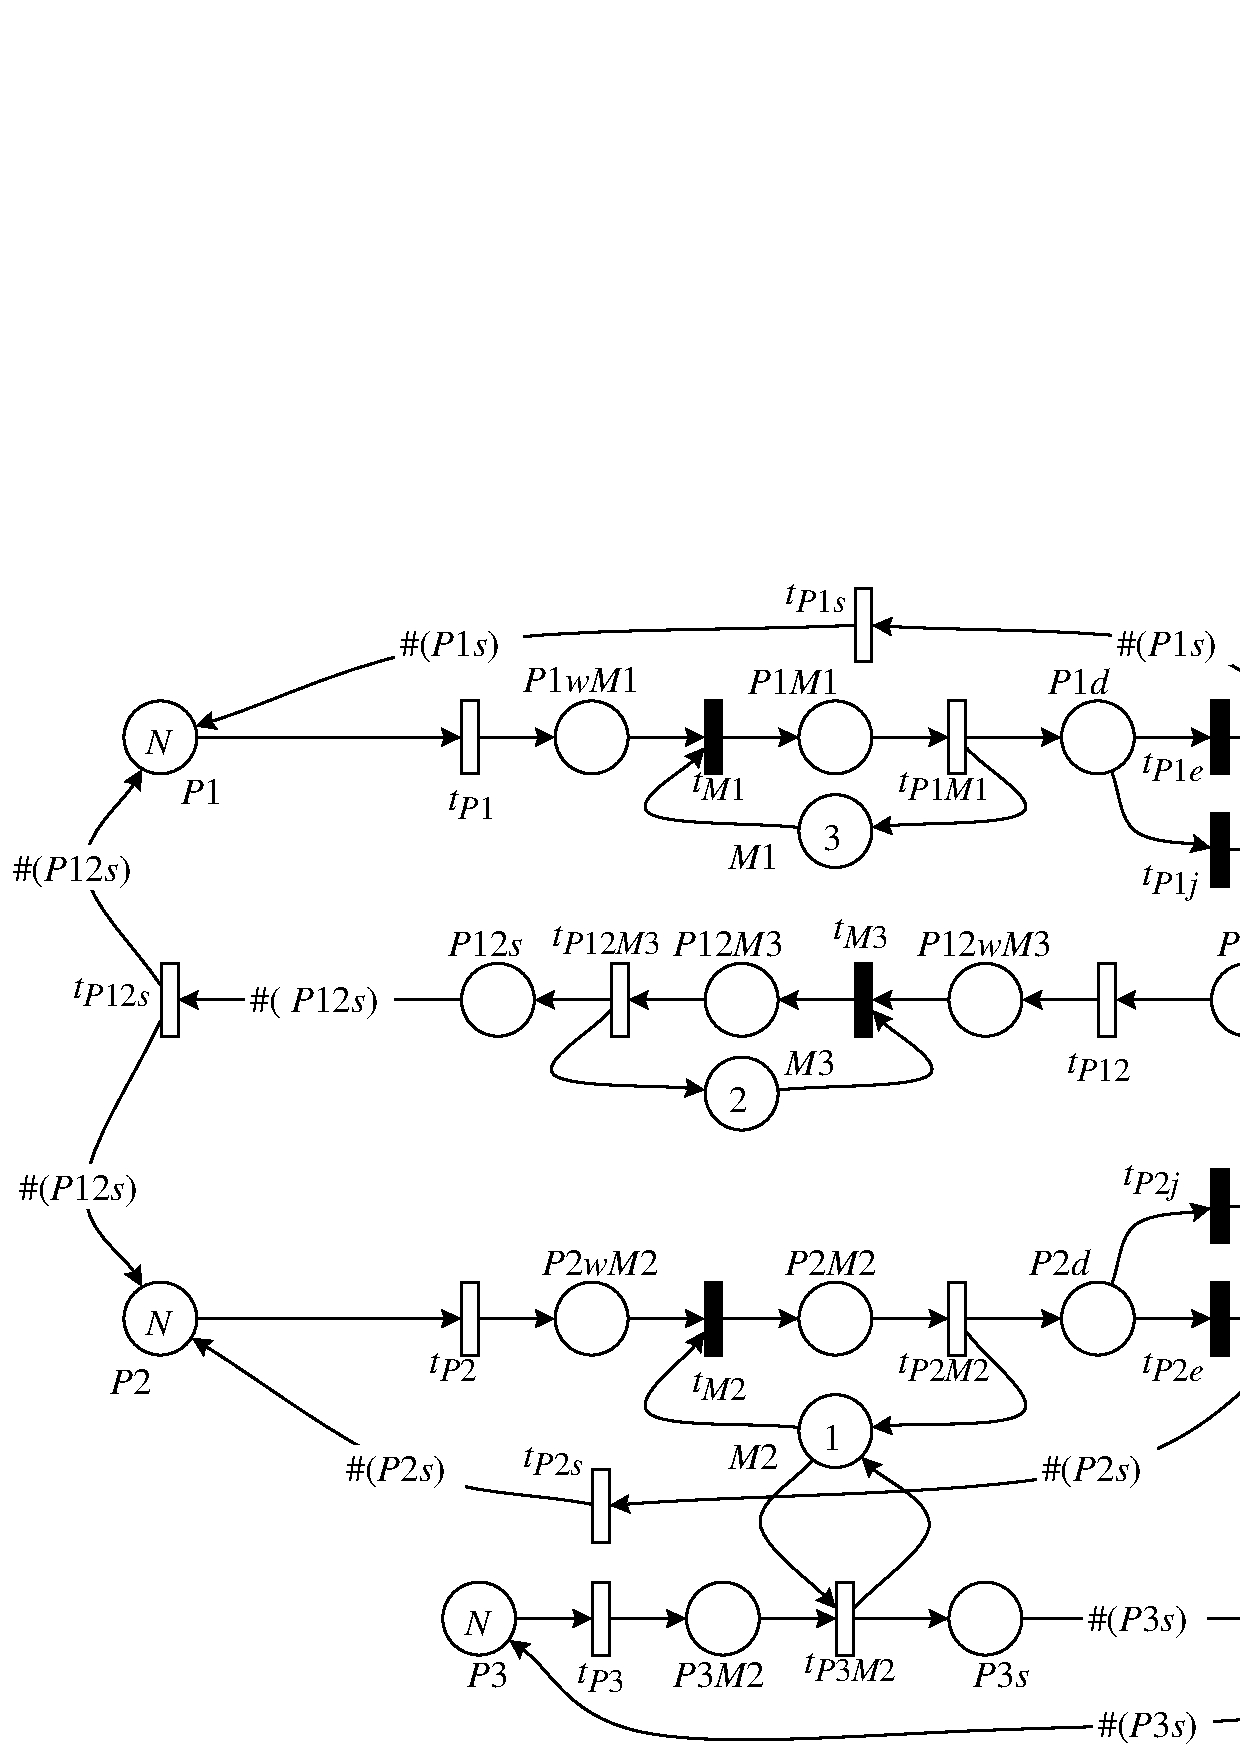
\includegraphics[scale=0.5]{figures/FMS-smartman.pdf}
  \caption{A flexible manufacturing system.}
  \label{FIG:fms}
\end{figure}


\begin{comment}

Had we wanted to use a structural solution approach, we could have
partitioned the model with the statement
\begin{code}
\begin{verbatim}
partition(P1:P1wM1:P1M1:M1:P1d:P1s, P12s:P12M3:M3:P12wM3:P12:P1wP2:P2wP1,
  P2:P2wM2:P2M2:M2:P2d:P2s, P3:P3M2:P3s);
\end{verbatim}
\end{code}
(which defines four submodels) and used the options
\begin{code}
\begin{verbatim}
# StateStorage MULTI_LEVEL_AVL
# MarkovStorage MATRIX_DIAGRAM_GENERAL
\end{verbatim}
\end{code}
Note, however, that the usually more efficient methods
\begin{code}
\begin{verbatim}
# StateStorage MDD_SATURATION
# MarkovStorage MATRIX_DIAGRAM_KRONECKER
\end{verbatim}
\end{code}
cannot be used with the given partition, because some immediate transitions,
such as \Code{tP1j}, are synchronizing (i.e., they affect multiple submodels).

%We partition the model into 19 levels obtained by assigning
%each place to a different level, with the exception of
%the complementary places $M_1$, $M_2$, and $M_3$, placed in the same level
%as the places $P_1M_1$, $P_2M_2$, and $P_{12}M_3$, respectively.

\end{comment}

%%%%%%%%%%%%%%%%%%%%%%%%%%%%%%%%%%%%%%%%%%%%%%%%%%%%%%%%%%%%%%%%%%%%%%%%%%%%
\section{Slotted ring}

Fig.~\ref{FIG:slotted} shows the Petri net for a single node of a slotted
ring network protocol \cite{Pastor1994}.
The overall model is composed of $N$
such subnets connected by merging transitions
(i.e., $\mathit{Free}_{(i+1) \bmod N}$ and $\mathit{Used}_{(i+1) \bmod N}$
really belong to the ``next'' subnet).
The following {\smart} code shows a decomposition where each
node of the ring is in a different level, and the requested
measure is simply the number of states.
%
\lstinputlisting[firstline=3]{examples/slot.sm}
%

\begin{figure}
  \centering
  \includegraphics[scale=0.5]{figures/slot.pdf}
  \caption{Model of a slotted ring.}
  \label{FIG:slotted}
\end{figure}


%%%%%%%%%%%%%%%%%%%%%%%%%%%%%%%%%%%%%%%%%%%%%%%%%%%%%%%%%%%%%%%%%%%%%%%%%%%%
\section{A Kanban system}

This model \cite{1996WMPN-SNSkanban}, shown in Fig.~\ref{FIG:kanban},
is parameterized by the number $N$ of tokens initially
in $p_{1}$, $p_{2}$, $p_{3}$, and $p_{4}$.
The following code shows a partition into four levels, one per kanban station.
The output measure is the number of arcs in the state-to-state transition
matrix for $N$ varying from $1$ to a maximum specified at runtime.
\begin{figure}
  \centering
  \includegraphics[scale=1]{figures/kanban.pdf}
  \caption{A kanban system.}
  \label{FIG:kanban}
\end{figure}
%
\lstinputlisting[firstline=3]{examples/kanban.sm}
%



%%%%%%%%%%%%%%%%%%%%%%%%%%%%%%%%%%%%%%%%%%%%%%%%%%%%%%%%%%%%%%%%%%%%%%%%%%%%
\section{Randomized leader election protocol}

The randomized asynchronous leader election protocol in \cite{DolevKR82}
solves the following problem: given a ring of $N$ processors, the
participants are required to designate a unique processor as leader by
sending messages around the ring. The ring is unidirectional, meaning that
the processes send messages to their unique successor (e.g. the one to the
right), and receive messages from their unique predecessor. It is known that
if the processors are indistinguishable (no unique identifiers are
assigned), then there is no deterministic algorithm to solve the problem.

The randomized algorithm works in phases. At the beginning of every round,
each process flips a coin to decide whether it will continue running for
election or not. Initially all processes are valid candidates. After
choosing a value ($0 = $ don't run this round, $1 = $ run), this is
communicated to the neighbour to the right. A process is eliminated from the
race only if it chose not to run and it's predecessor chose to run. After
being eliminated from the race, a process never becomes eligible again (it
enters the inactive state), and it is used only to relay messages between
active nodes around the ring. They do no initiate any communication.
Termination is detected by the active processes (at least one active node
exists at all times) by sending a token around the ring to count the
inactive nodes. The process that receives its own token with count $N-1$ is
the elected leader.

In our model, each processes has $5$ state variables:
\begin{lstlisting}
status[i]       : {start, wait, active, inactive, leader};      // init start
preference[i]   : {0, 1};                                       // init 0
counter[i]      : {0..N-1};                                     // init 0
sent[i]         : {none, pref, counter};                        // init none
recv[i]         : {none, pref, counter};                        // init none
\end{lstlisting}

\begin{figure}
  \centering
  \includegraphics[scale=0.5]{figures/leaderchart.pdf}
  \caption{State transition chart for the \Code{status} variable.}
  \label{FIG:leaderchart}
\end{figure}

\noindent The state-transition diagram for the \Code{status} of a process is
shown in Figure \ref{FIG:leaderchart}.

\IGNORE{
The Petri Net model is shown is Figure \ref{FIG:leaderfig}
\begin{figure}
  \CENTERPSSCALE{leaderfig}{0.5}
  \caption{Petri net model: the subnet of process $i$.}
  \label{FIG:leaderfig}
\end{figure}
}

\noindent The SMART code for this model is listed below:
%
\lstinputlisting[firstline=3]{examples/leader.sm}
%



%%%%%%%%%%%%%%%%%%%%%%%%%%%%%%%%%%%%%%%%%%%%%%%%%%%%%%%%%%%%%%%%%%%%%%%%%%%%
\section{A round--robin mutual exclusion protocol}

\begin{comment}
The protocol regulates the access to a shared resource (e.g. a communication
channel) for a ring of $N$ processors. The resource manager gives permission
to use the channel to each process in order, by moving a token around the
ring. When a process has the token, it reads in a message from the channel and
stores it in its own buffer. It can then release the token to the next processor 
before reading the contents of the buffer, or read the buffer first and then 
send the token to the neighbour.

Figure \ref{FIG:robinfig} shows the subnet for process $i$. 
Each subnet is initially marked with one token in place $\id{wait}_i$, 
except for process $0$ which starts with one token in $\id{req}_i$, meaning 
that it is the first process to have access when the protocol starts.

\begin{figure}
  \CENTERPSSCALE{robinfig}{0.5}
  \caption{The round--robin mutual exclusion.}
  \label{FIG:robinfig}
\end{figure}

\begin{code}
\begin{verbatim}
spn robin(int N) := {
  place Res;
  partition(1:Res);
  for (int i in {0..N-1}) {
    place
        R[i], bufidle[i], buffull[i],
        pwait[i], pask[i], pok[i], pload[i], psend[i];
    trans
        task[i], tbuf[i], t1load[i], t2load[i], t1send[i], t2send[i];
    partition(
        i+2:bufidle[i]:buffull[i]:pwait[i]:pask[i]:pok[i]:pload[i]:psend[i],
        1:R[i]);
    firing(task[i]:expo(1.0), tbuf[i]:expo(1.0), t1load[i]:expo(1.0),
        t1send[i]:expo(1.0), t2load[i]:expo(1.0), t2send[i]:expo(1.0));
  }
  for (int i in {0..N-1}) {
    arcs(Res:task[i], pask[i]:task[i], task[i]:R[i], task[i]:pok[i],
        R[i]:tbuf[i], bufidle[i]:tbuf[i], tbuf[i]:buffull[i], tbuf[i]:Res,
        buffull[i]:t1load[i], pok[i]:t1load[i], t1load[i]:bufidle[i], t1load[i]:psend[i],
        buffull[i]:t2load[i], pload[i]:t2load[i], t2load[i]:bufidle[i], t2load[i]:pwait[i],
        pok[i]:t1send[i], pwait[mod(i+1,N)]:t1send[i], 
        t1send[i]:pload[i], t1send[i]:pask[mod(i+1,N)],
        psend[i]:t2send[i], pwait[mod(i+1,N)]:t2send[i], 
        t2send[i]:pwait[i], t2send[i]:pask[mod(i+1,N)]);
  }
  init(Res:1, pask[0]:1);
  for (int i in {1..N-1}) {init (pwait[i]:1);}
  for (int i in {0..N-1}) {init(bufidle[i]:1);}
}
\end{verbatim}
\end{code}

\end{comment}
